\section{Controlled Comparison and Sensitivity Study}
\subsection{Experimental Protocol}
To compare steering methods with a common speed policy, we extended the local F1TENTH controller with a Pure Pursuit branch \cite{coulter1992pursuit}. Its target is interpolated 1.5~m ahead in centerline arc length and its steering law is
\begin{equation}
\delta_{\mathrm{PP}}=\operatorname{atan2}\!\left(\frac{2L y_g}{x_g^2+y_g^2},1\right),
\end{equation}
where $(x_g,y_g)$ is the target in the vehicle frame and $L=0.3302$~m. Both branches use the same curvature- and forward-distance-based speed command, a 7.0~m/s speed ceiling, $\pm0.4189$~rad steering limit, and 3.2~rad/s steering slew limit. This isolates the steering choice more closely than comparing two independently tuned speed planners; it does not test a globally optimized racing policy. The RMPC branch retains its original weights, 100-stage horizon, 20~ms prediction step and seven basis coefficients. We varied only the number of sampled trajectories: 1,000, 2,500 and 5,000.

The test harness calls the actual compiled C++/CUDA controller through a synchronous stream. It passes the current ground-truth vehicle state and 819-beam LiDAR scan, waits for one steering/speed command, then advances F1TENTH Gym by two 10~ms RK4 physics steps. Thus the control period is exactly 20~ms in simulation time, independent of wall-clock execution. This design measures computational cost without ROS transport, GUI rendering or simulator time in the timed region. A monotonic timer encloses the synchronized RMPC \texttt{solve()} call, including GPU sampling, rollout, transfers and host-side selection; it is not GPU-kernel-only time. A second timer covers perception, controller callback and publication. The first simulated second is omitted from steady timing summaries, while all states remain in the lap and tracking metrics. These computation times should not be conflated with the earlier asynchronous ROS \texttt{/drive} intervals.

We ran ten independent restarts per method and map, with paired seeds 81000--81009 and randomized run order: 80 nominal trials. Each trial starts near centerline point 0 from rest, with lateral perturbation $\mathcal N(0,0.05^2)$~m clipped to $\pm0.12$~m and yaw perturbation $\mathcal N(0,0.01^2)$~rad clipped to $\pm0.03$~rad. LiDAR range noise has 0.01~m standard deviation; ground-truth odometry is supplied. Each run ends on a Gym collision, completion of one unwrapped centerline length, or a 180~s simulated-time limit. Root-mean-square (RMS) $d$ uses all state samples in the trial. Lap time is reported only after completion. A separate repeat of the pilot seed reproduced the state and command sequence exactly; pilot seed 70001 was excluded from the study.

The simulator's nominal F1TENTH body has mass 3.74~kg, friction coefficient 1.0489 and width 0.31~m. The inherited RMPC prediction model uses 3.47~kg, 0.523 and 0.2032~m; these model differences are retained. The archived controller YAML, simulator settings, map and centerline hashes, source-script and binary hashes, per-step traces, run order and numerical summaries are in the accompanying \texttt{RMPC\_F1TENTH/experiments} folder. The controlled traces are \texttt{NPZ} arrays; the earlier ROS~2 bags are a separate dataset.

\subsection{Nominal Results and Sample Count}
All 80 nominal trials completed one lap without a Gym collision. Table~\ref{tab:controlled} reports the ten-trial mean and sample standard deviation, and Fig.~\ref{fig:controlled} shows each trial. On both maps, the selected Pure Pursuit baseline has lower RMS centerline error and mean lap time than the 5,000-sample RMPC under the shared speed policy. Pairing by seed, RMPC minus Pure Pursuit RMS error averages 0.142~m on IMS (95\% paired bootstrap interval 0.128--0.156~m) and 0.213~m on the new circuit (0.201--0.223~m). Corresponding paired lap-time differences are 3.68~s (2.42--4.86~s) and 2.23~s (1.11--3.49~s). These bootstrap intervals resample ten seed pairs 10,000 times; they describe uncertainty under the narrow perturbation protocol, not general controller ranking. A 10/10 completion count does not imply a zero failure probability on unseen tracks.

\begin{table*}[t]
\centering\small
\caption{Fixed 50 Hz study, ten independent trials per row. Means $\pm$ sample SD are over trials; lap time is reported for completed trials. P99 is calculated within each trial and then averaged.}
\label{tab:controlled}
\begin{tabular}{llrrrr}
\toprule
Track & Controller & Completed & Lap (s) & RMS $d$ (m) & Pipeline P99 (ms)\\
\midrule
IMS & Pure Pursuit & 10/10 & 49.83 $\pm$ 0.03 & 0.042 $\pm$ 0.001 & 0.144 $\pm$ 0.056 \\
IMS & RMPC 1000 & 10/10 & 55.04 $\pm$ 1.33 & 0.218 $\pm$ 0.015 & 1.267 $\pm$ 0.098 \\
IMS & RMPC 2500 & 10/10 & 55.98 $\pm$ 2.43 & 0.214 $\pm$ 0.033 & 1.256 $\pm$ 0.075 \\
IMS & RMPC 5000 & 10/10 & 53.51 $\pm$ 2.09 & 0.184 $\pm$ 0.024 & 1.308 $\pm$ 0.103 \\
New circuit & Pure Pursuit & 10/10 & 58.92 $\pm$ 0.05 & 0.056 $\pm$ 0.001 & 0.145 $\pm$ 0.057 \\
New circuit & RMPC 1000 & 10/10 & 62.62 $\pm$ 2.72 & 0.312 $\pm$ 0.033 & 1.288 $\pm$ 0.137 \\
New circuit & RMPC 2500 & 10/10 & 61.22 $\pm$ 1.62 & 0.278 $\pm$ 0.019 & 1.265 $\pm$ 0.101 \\
New circuit & RMPC 5000 & 10/10 & 61.16 $\pm$ 2.01 & 0.269 $\pm$ 0.018 & 1.266 $\pm$ 0.101 \\
\bottomrule
\end{tabular}
\end{table*}


\begin{figure*}[t]
\centering
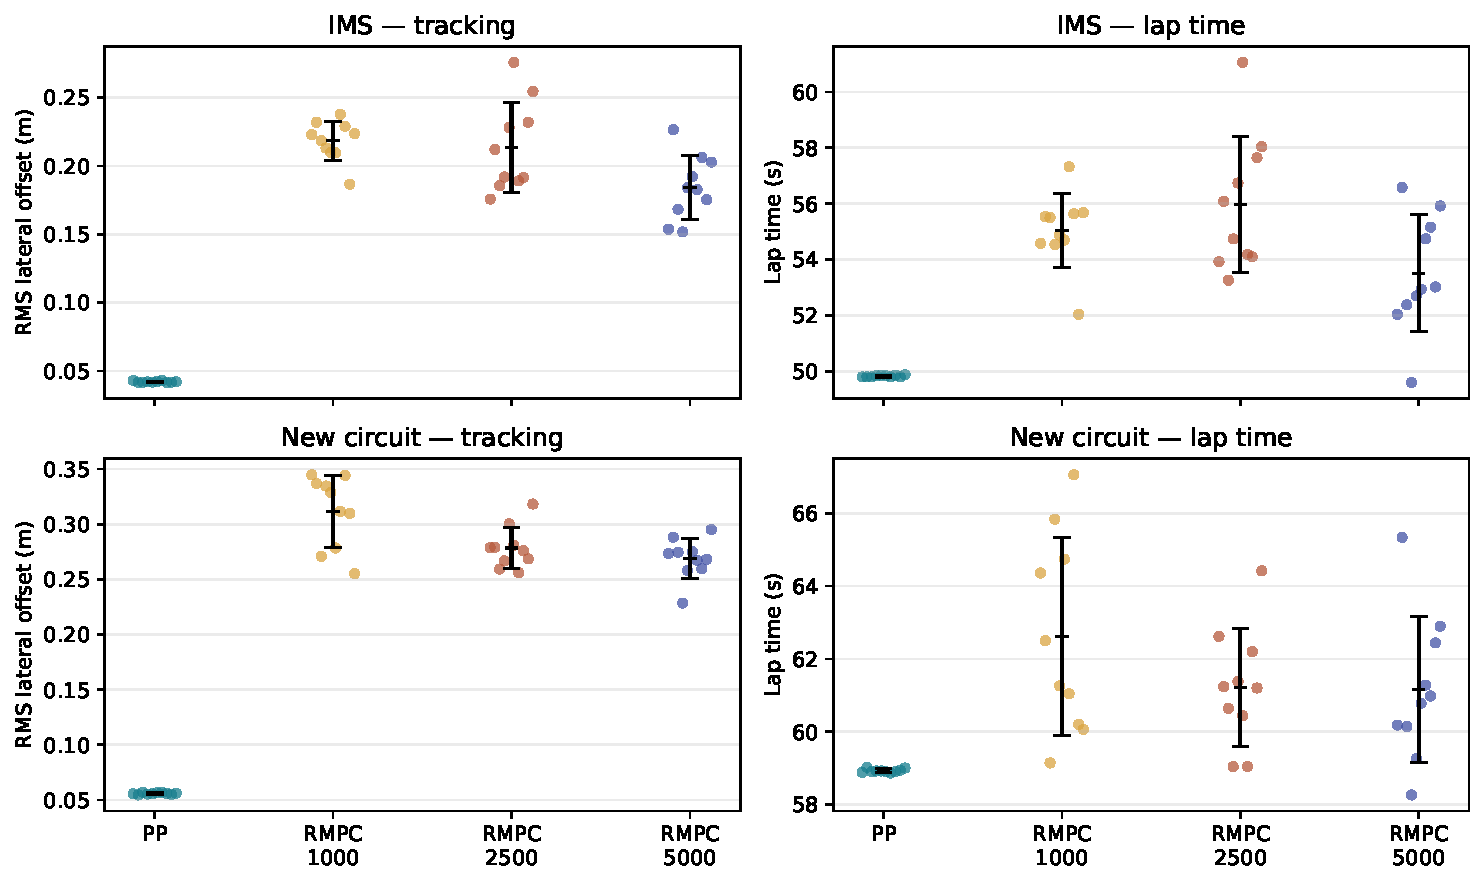
\includegraphics[width=.88\textwidth]{figures/controlled_comparison.pdf}
\caption{Ten independent nominal trials per condition. Dots are trial outcomes; black bars are mean and sample standard deviation. PP denotes Pure Pursuit. All 80 runs completed; the figure retains every lap and RMS offset.}
\label{fig:controlled}
\end{figure*}

Figure~\ref{fig:samples} shows that increasing RMPC samples from 1,000 to 5,000 changed the mean median synchronized solve-call duration only modestly: 0.881 to 0.919~ms on IMS and 0.886 to 0.919~ms on the new circuit. Mean RMS offset declined from 0.218 to 0.184~m on IMS and 0.312 to 0.269~m on the new circuit, but the 2,500-sample trial outcomes and lap times were not monotonic. Fixed transfer, synchronization and selection costs contribute to the measured call duration. Across all 100 controlled trials, the largest individual RMPC solve call was 5.72~ms. No observed solve call exceeded 20~ms in this unloaded synchronous harness; that fact alone does not establish an asynchronous ROS deadline guarantee.

\begin{figure*}[t]
\centering
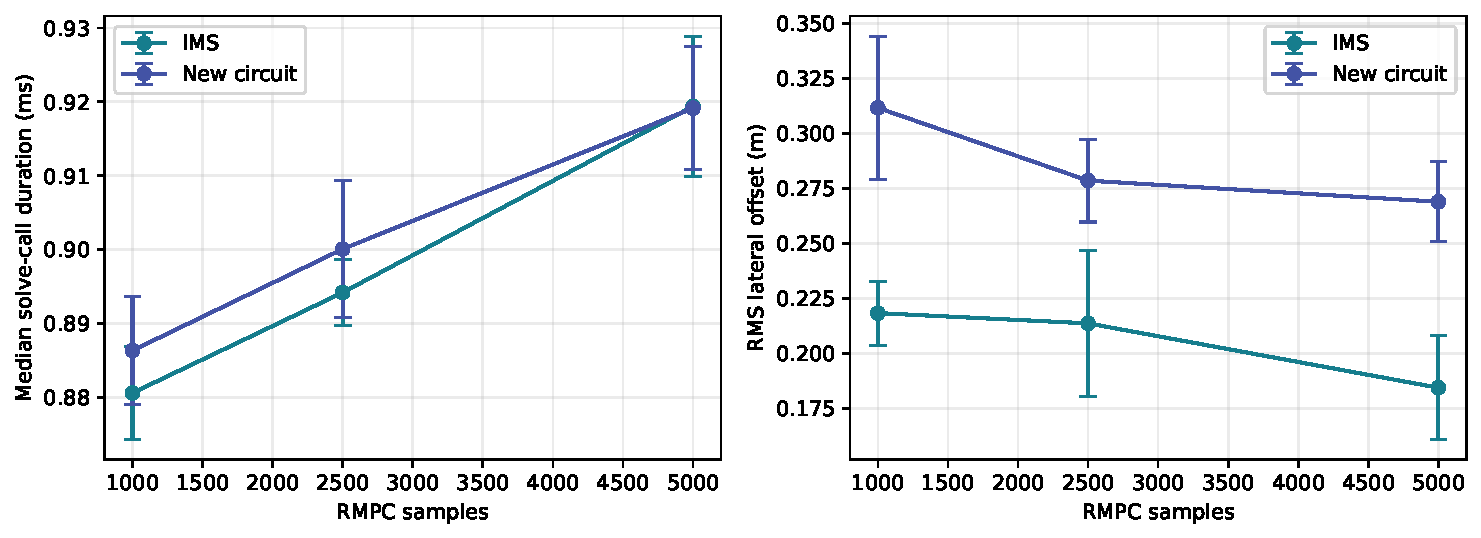
\includegraphics[width=.83\textwidth]{figures/sample_tradeoff.pdf}
\caption{RMPC sample-count sensitivity. Points are ten-trial means; bars show sample standard deviation across trial-level median solve durations (left) and RMS lateral errors (right). The timed solve call includes synchronized GPU work and CPU selection.}
\label{fig:samples}
\end{figure*}

\subsection{Unannounced Low-Grip Sector}
For a separate robustness probe, we repeated the new-circuit comparison at 5,000 RMPC samples with the same ten paired seeds. The simulator's friction coefficient drops from 1.0489 to 0.35 between 15\% and 35\% of centerline progress, then returns to 1.0489. Neither controller is informed of the change; RMPC's assumed coefficient stays at 0.523. All 20 runs completed without a Gym collision or center crossing beyond the nominal map half-width. Mean RMS $d$ rose from 0.056 to 0.145~m for Pure Pursuit and from 0.269 to 0.334~m for RMPC. Mean laps changed from 58.92 to 59.19~s and from 61.16 to 61.75~s, respectively. Figure~\ref{fig:slippery} shows the preselected seed 81000, with the affected sector shaded. The sector models an abrupt parameter change; it does not model water, changing tire temperature or sensor delay. The absence of failures in ten trials per method is limited evidence of robustness.

\begin{figure*}[t]
\centering
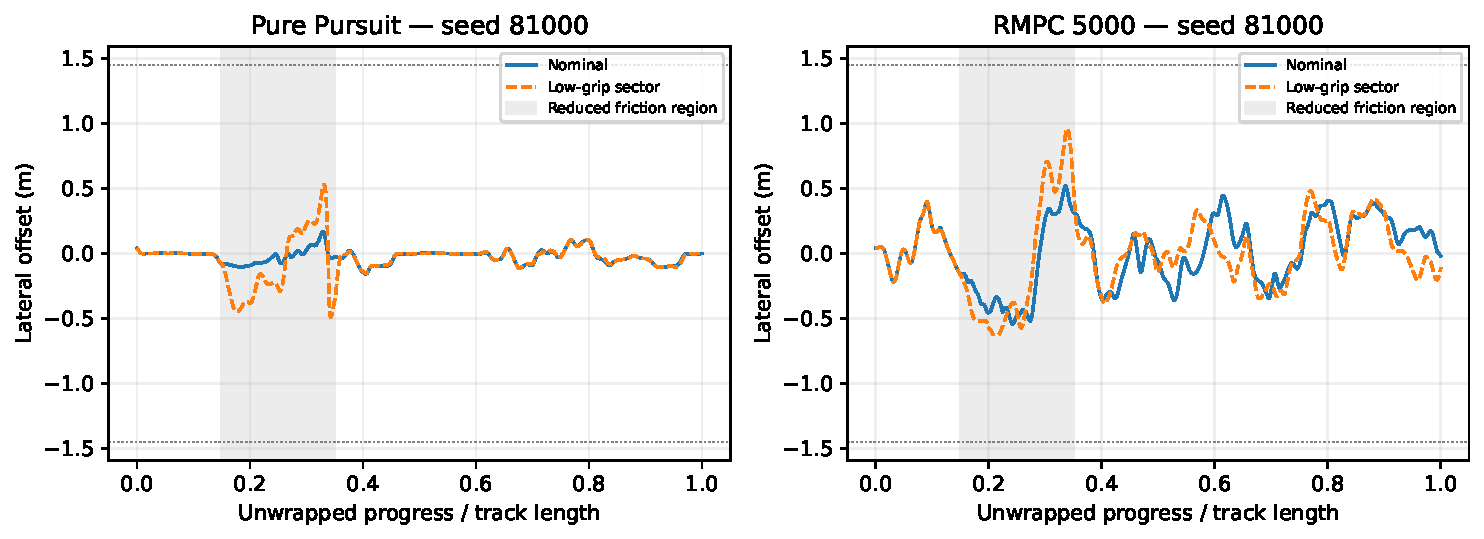
\includegraphics[width=.83\textwidth]{figures/slippery_response.pdf}
\caption{Nominal and reduced-grip lateral responses for the predetermined seed 81000. The shaded interval is the simulator's low-grip sector ($\mu=0.35$). Dotted lines show the new circuit's 1.45~m centerline-to-map-edge distance, not full-body clearance.}
\label{fig:slippery}
\end{figure*}
